% !TEX TS-program = pdflatex
% !TEX encoding = UTF-8 Unicode

% This file is a template using the "beamer" package to create slides for a talk or presentation


\documentclass[xcolor=table]{beamer}
\usepackage{setspace}
 \usepackage{tabularx} 
\usepackage{arydshln}
%\setbeamersize{text margin left=5pt,text margin right=5pt}
%\definecolor{LRed}{rgb}{1,.8,.8}
%\definecolor{MRed}{rgb}{1,.6,.6}
\definecolor{HRed}{rgb}{1,.2,.2}
\usepackage{mathtools}

\setbeamertemplate{footline}[frame number]
\mode<presentation>
{
  \usetheme{Darmstadt}
  % or ...

  \setbeamercovered{transparent}
  % or whatever (possibly just delete it)
}

\usepackage{tikz}
%\usepackage{chronosys}
\usepackage{breqn}

\usepackage{bbm}
\usepackage[english]{babel}
% or whatever
\usepackage{color,soul}
\usepackage[utf8]{inputenc}
% or whatever
\usepackage{color, colortbl}
\usepackage{times}
\usepackage[T1]{fontenc}
% Or whatever. Note that the encoding and the font should match. If T1
% does not look nice, try deleting the line with the fontenc.
\newcommand\tab[1][1cm]{\hspace*{#1}}
\usepackage{xcolor}


\newcommand\Wider[2][4em]{%
\makebox[\linewidth][c]{%
  \begin{minipage}{\dimexpr\textwidth+#1\relax}
  \raggedright#2
  \end{minipage}%
  }%
}

\newcommand{\highlight}[1]{%
  \colorbox{yellow!50}{$\displaystyle#1$}}
\title[Effects of a Minimum Wage Increase on Restaurants] % (optional, use only with long paper titles)
{\large Minimum Wage Project: \\ Means and Results}

%\subtitle
%{Include Only If Paper Has a Subtitle}

\author[Chelsea Crain] % (optional, use only with lots of authors)
{}
% - Give the names in the same order as the appear in the paper.
% - Use the \inst{?} command only if the authors have different
%   affiliation.

\institute[] % (optional, but mostly needed)


\date % (optional, should be abbreviation of conference name)
{Chelsea Crain\\
University of Iowa\\
\today \\

}



\begin{document}



\begin{spacing}{1.2}
\begin{frame}
  \titlepage
\end{frame}

\begin{frame}{General Pass Through Geo}
\Wider{
\centering
\tiny
\begin{center}
\begin{tabular}{lcccccccc}
\hline  & \multicolumn{5}{c}{Yelp} & \multicolumn{3}{c}{Grubhub}\\
 & (1) & (2) & (3) & (4) & (5) & (6) & (7) & (8)\\
 & All & Cntrls & Change & Eat24 & Eat24+GH & All & Cntrls & Eat24\\
\hline  $ Jul16-Oct16 $  & 0.084 & 0.023 & 0.378 & 0.313 & -0.236 &  &  & \\
 & (0.040) & (0.067) & (0.178) & (0.212) & (0.418) &  &  & \\
 $ Oct16-Jan17 $  & 0.171*** & 0.185** & 0.668** & 0.326** & -0.235 &  &  & \\
 & (0.034) & (0.064) & (0.198) & (0.114) & (0.334) &  &  & \\
 $ Jan17-Apr17 $  & 0.162*** & 0.148* & 0.556* & 0.272 & 0.625 &  &  & \\
 & (0.034) & (0.059) & (0.202) & (0.183) & (0.339) &  &  & \\
\hline  $ Dec16-Jan17 $  &  &  &  &  &  & 0.260*** & 0.271*** & 0.206***\\
 &  &  &  &  &  & (0.010) & (0.007) & (0.022)\\
 $ Jan17-Feb17 $  &  &  &  &  &  & 0.245*** & 0.293*** & 0.149**\\
 &  &  &  &  &  & (0.042) & (0.028) & (0.044)\\
 $ Feb17-Mar17 $  &  &  &  &  &  & 0.244*** & 0.295*** & 0.209***\\
 &  &  &  &  &  & (0.022) & (0.015) & (0.044)\\
 $ Mar17-Apr17 $  &  &  &  &  &  & 0.162*** & 0.161*** & 0.032\\
 &  &  &  &  &  & (0.013) & (0.023) & (0.087)\\
\hline \textit{Total Pass Through} & 0.333*** & 0.333*** & 1.224***+ & 0.598** & 0.39 & 0.911*** & 1.019***+ & 0.596***\\
  & (0.066) & (0.114) & (0.394) & (0.281) & (0.434) & (0.053) & (0.069) & (0.166)\\
\hline  $ N $  & 8805 & 5257 & 2099 & 2269 & 432 & 3653 & 2760 & 432\\
 $ NxT $  & 35220 & 21028 & 8396 & 9076 & 1728 & 14612 & 11040 & 1728\\
\hline\end{tabular}\\
\begin{tiny}p<0.1; ** $p<0$.05; *** $p<0$.01; + statistically different than column (1) \end{tiny}\\
\end{center}

}
\end{frame}

\begin{frame}{General Pass Through Geo}
\Wider{
\centering
\tiny
<<<<<<< HEAD
\begin{center}
\begin{tabular}{lcccccc}
\hline  & (1) & (2) & (3) & (4) & (5) & (6)\\
 & Low Sales & High Sales & Low Emps & High Emps & Low Stars & High Stars\\
\hline  $ Apr16-Jul16 $  & 0.288 & 0.182 & 0.249 & 0.122 & 0.189 & 0.026\\
 & (0.145) & (0.271) & (0.147) & (0.260) & (0.076) & (0.114)\\
 $ Jul16-Oct16 $  & 0.249 & -0.073 & 0.286 & 0.019 & 0.260 & 0.153\\
 & (0.182) & (0.204) & (0.140) & (0.245) & (0.056) & (0.126)\\
 $ Oct16-Jan17 $  & 0.260 & 0.096 & 0.364 & 0.032 & 0.429 & 0.189\\
 & (0.126) & (0.121) & (0.119) & (0.155) & (0.033) & (0.080)\\
 $ Jan16-Apr17 $  & 0.468 & 0.334 & 0.238 & 0.386 & 0.361 & 0.190\\
 & (0.122) & (0.142) & (0.132) & (0.176) & (0.094) & (0.103)\\
\hline \textit{Total Pass Through} & 0.728 & 0.43 & 0.602$^+$ & 0.418$^+$ & 0.79 & 0.379\\
  & (0.244) & (0.262) & (0.231) & (0.331) & (0.119) & (0.183)\\
\hline  $ N $  & 1556 & 1723 & 2142 & 1894 & 3832 & 6783\\
 $ NxT $  & 6224 & 6892 & 8568 & 7576 & 15328 & 27132\\
\hline\end{tabular}\\
\begin{tiny} + statistically different than comparison group \end{tiny}\\
\end{center}
=======
\begin{center}
\begin{tabular}{lcccccc}
\hline  & (1) & (2) & (3) & (4) & (5) & (6)\\
 & Low Sales & High Sales & Low Emps & High Emps & Low Stars & High Stars\\
\hline  $ Apr16-Jul16 $  & 0.288 & 0.182 & 0.249 & 0.122 & 0.189 & 0.026\\
 & (0.145) & (0.271) & (0.147) & (0.260) & (0.076) & (0.114)\\
 $ Jul16-Oct16 $  & 0.249 & -0.073 & 0.286 & 0.019 & 0.260 & 0.153\\
 & (0.182) & (0.204) & (0.140) & (0.245) & (0.056) & (0.126)\\
 $ Oct16-Jan17 $  & 0.260 & 0.096 & 0.364 & 0.032 & 0.429 & 0.189\\
 & (0.126) & (0.121) & (0.119) & (0.155) & (0.033) & (0.080)\\
 $ Jan16-Apr17 $  & 0.468 & 0.334 & 0.238 & 0.386 & 0.361 & 0.190\\
 & (0.122) & (0.142) & (0.132) & (0.176) & (0.094) & (0.103)\\
\hline \textit{Total Pass Through} & 0.728 & 0.43 & 0.602$^+$ & 0.418$^+$ & 0.79 & 0.379\\
  & (0.244) & (0.262) & (0.231) & (0.331) & (0.119) & (0.183)\\
\hline  $ N $  & 1556 & 1723 & 2142 & 1894 & 3832 & 6783\\
 $ NxT $  & 6224 & 6892 & 8568 & 7576 & 15328 & 27132\\
\hline\end{tabular}\\
\begin{tiny} + statistically different than comparison group \end{tiny}\\
\end{center}
>>>>>>> 9bf80c4d3367c601bceb3268e37dc31cf9116a6c

}
\end{frame}

\begin{frame}{Pass Through: Rest Chars Yelp Geo}
\Wider{
\centering
\tiny
{
\def\sym#1{\ifmmode^{#1}\else\(^{#1}\)\fi}
\begin{tabular}{l*{6}{c}}
\hline\hline
                    &\multicolumn{1}{c}{(1)}&\multicolumn{1}{c}{(2)}&\multicolumn{1}{c}{(3)}&\multicolumn{1}{c}{(4)}&\multicolumn{1}{c}{(5)}&\multicolumn{1}{c}{(6)}\\
                    &\multicolumn{1}{c}{Low Sales}&\multicolumn{1}{c}{High Sales}&\multicolumn{1}{c}{Low Emps}&\multicolumn{1}{c}{High Emps}&\multicolumn{1}{c}{Low Stars}&\multicolumn{1}{c}{High Stars}\\
\hline
$ Jul-Oct $         &     -0.0849         &      -0.164         &       0.462         &     -0.0870         &      -0.182         &     -0.0284         \\
                    &    (0.0790)         &     (0.137)         &     (0.315)         &     (0.152)         &     (0.104)         &    (0.0978)         \\
[1em]
$ Oct-Jan $         &      0.0701         &     -0.0180         &       0.480\sym{*}  &     -0.0153         &       0.141         &      0.0135         \\
                    &    (0.0663)         &    (0.0888)         &     (0.220)         &     (0.100)         &    (0.0924)         &    (0.0648)         \\
[1em]
$ Jan-Apr $         &       0.121\sym{**} &       0.330\sym{**} &       0.503         &       0.323\sym{**} &       0.208         &     -0.0335         \\
                    &    (0.0397)         &     (0.101)         &     (0.246)         &     (0.109)         &     (0.115)         &     (0.110)         \\
\hline
Observations        &        5332         &        5960         &        5940         &        7368         &        5376         &       10676         \\
\hline\hline
\multicolumn{7}{l}{\footnotesize Standard errors in parentheses}\\
\multicolumn{7}{l}{\footnotesize \sym{*} \(p<.10\), \sym{**} \(p<.05\), \sym{***} \(p<.001\)}\\
\end{tabular}
}

}
\end{frame}


\begin{frame}{General Pass Through Yelp Geo}
\Wider{
\centering
\tiny
{
\def\sym#1{\ifmmode^{#1}\else\(^{#1}\)\fi}
\begin{tabular}{l*{5}{c}}
\hline\hline
                    &\multicolumn{1}{c}{(1)}&\multicolumn{1}{c}{(2)}&\multicolumn{1}{c}{(3)}&\multicolumn{1}{c}{(4)}&\multicolumn{1}{c}{(5)}\\
                    &\multicolumn{1}{c}{(mean) ch\_lnp}&\multicolumn{1}{c}{(mean) ch\_lnp}&\multicolumn{1}{c}{(mean) ch\_lnp}&\multicolumn{1}{c}{(mean) ch\_lnp}&\multicolumn{1}{c}{(mean) ch\_lnp}\\
\hline
 $ Apr-Jul $        &      0.0461         &      0.0832\sym{**} &       0.310\sym{**} &      0.0120         &       0.111         \\
                    &    (0.0294)         &    (0.0215)         &     (0.114)         &     (0.143)         &     (0.339)         \\
[1em]
 $ Jul-Oct $        &       0.115         &      0.0764         &       0.639\sym{**} &     -0.0108         &      -0.296         \\
                    &    (0.0698)         &    (0.0726)         &     (0.192)         &     (0.280)         &     (0.678)         \\
[1em]
 $ Oct-Jan $        &       0.191\sym{**} &       0.202\sym{**} &       0.451\sym{**} &     -0.0695         &       0.105         \\
                    &    (0.0483)         &    (0.0573)         &     (0.127)         &     (0.136)         &     (0.361)         \\
[1em]
 $ Jan-Apr $        &       0.157\sym{**} &       0.142\sym{*}  &       0.435\sym{**} &       0.368         &       0.408         \\
                    &    (0.0602)         &    (0.0556)         &     (0.131)         &     (0.192)         &     (0.483)         \\
\hline
Observations        &       35460         &       21204         &        9080         &        4368         &        2468         \\
\hline\hline
\multicolumn{6}{l}{\footnotesize Standard errors in parentheses}\\
\multicolumn{6}{l}{\footnotesize \sym{*} \(p<.10\), \sym{**} \(p<.05\), \sym{***} \(p<.001\)}\\
\end{tabular}
}

}
\end{frame}


\begin{frame}{General Pass Through RUSA}
\Wider{
\centering
\tiny
{
\def\sym#1{\ifmmode^{#1}\else\(^{#1}\)\fi}
\begin{tabular}{c*{5}{c}}
\hline\hline
					& \multicolumn{3}{c}{Yelp} & \multicolumn{2}{c}{Grubhub} \\ \cline{2-4} \cline{5-6}
                   % &\multicolumn{1}{c}{(1)}         &\multicolumn{1}{c}{(2)}         &\multicolumn{1}{c}{(3)}         &\multicolumn{1}{c}{(4)}         &\multicolumn{1}{c}{(5)}         \\
                    &        All         &      Cntrls         &      Change         &        All         &        Cntrls        \\
\hline
 $ Jul-Oct $        &       0.183\sym{***}&       0.173\sym{*}  &       0.398         &                     &                     \\
                    &    (0.0317)         &    (0.0808)         &     (0.244)         &                     &                     \\
[1em]
 $ Oct-Jan $        &       0.197\sym{**} &       0.189         &       0.355         &                     &                     \\
                    &    (0.0644)         &     (0.104)         &     (0.373)         &                     &                     \\
[1em]
 $ Jan-Apr $        &       0.270\sym{***}&       0.244\sym{**} &       0.636\sym{**} &                     &                     \\
                    &    (0.0424)         &    (0.0667)         &     (0.140)         &                     &                     \\
[1em]
 $ Dec-Jan $        &                     &                     &                     &       0.181\sym{***}&       0.207\sym{***}\\
                    &                     &                     &                     &   (0.00969)         &    (0.0108)         \\
[1em]
 $ Jan-Feb $        &                     &                     &                     &       0.266\sym{***}&       0.273\sym{***}\\
                    &                     &                     &                     &    (0.0400)         &    (0.0406)         \\
[1em]
 $ Feb-Mar $        &                     &                     &                     &       0.272\sym{***}&       0.312\sym{***}\\
                    &                     &                     &                     &    (0.0210)         &    (0.0455)         \\
[1em]
 $ Mar-Apr $        &                     &                     &                     &       0.188\sym{**} &       0.193\sym{**} \\
                    &                     &                     &                     &    (0.0587)         &    (0.0706)         \\
\hline
Total Pass Through & 0.65 & 0.606 & 1.39 & 0.91 & 0.985 \\
N & 7283 & 6830 & 1786 & 3935 & 3561 \\
N x T        &       29132         &       27320         &        7144         &       15740         &       14244         \\
\hline\hline
%\multicolumn{6}{l}{\footnotesize Standard errors in parentheses}\\
\multicolumn{6}{l}{\tiny \sym{*} \(p<.10\), \sym{**} \(p<.05\), \sym{***} \(p<.001\)}\\
\end{tabular}
}

}
\end{frame}


\begin{frame}{Pass Through: Rest Chars Yelp RUSA}
\Wider{
\centering
\tiny
{
\def\sym#1{\ifmmode^{#1}\else\(^{#1}\)\fi}
\begin{tabular}{l*{6}{c}}
\hline\hline
                    &\multicolumn{1}{c}{(1)}&\multicolumn{1}{c}{(2)}&\multicolumn{1}{c}{(3)}&\multicolumn{1}{c}{(4)}&\multicolumn{1}{c}{(5)}&\multicolumn{1}{c}{(6)}\\
                    &\multicolumn{1}{c}{Low Sales}&\multicolumn{1}{c}{High Sales}&\multicolumn{1}{c}{Low Emps}&\multicolumn{1}{c}{High Emps}&\multicolumn{1}{c}{Low Stars}&\multicolumn{1}{c}{High Stars}\\
\hline
$ Oct-Jan $         &     0.00202         &       0.131\sym{*}  &      0.0978         &      0.0668\sym{*}  &      0.0242         &      0.0526         \\
                    &     (0.115)         &    (0.0402)         &     (0.153)         &    (0.0248)         &     (0.131)         &    (0.0270)         \\
[1em]
$ Jan-Apr$          &      0.0222         &       0.374\sym{***}&       0.324         &       0.361\sym{***}&       0.715         &      0.0405         \\
                    &     (0.119)         &    (0.0699)         &     (0.183)         &    (0.0474)         &     (0.362)         &    (0.0601)         \\
\hline
Observations        &        6124         &        8824         &        3416         &        9116         &        3216         &       13996         \\
\hline\hline
\multicolumn{7}{l}{\footnotesize Standard errors in parentheses}\\
\multicolumn{7}{l}{\footnotesize \sym{*} \(p<0.05\), \sym{**} \(p<0.01\), \sym{***} \(p<0.001\)}\\
\end{tabular}
}

}
\end{frame}

\begin{frame}{Pass Through: Item Chars GH Geo}
\Wider{
\centering
\tiny
{
\def\sym#1{\ifmmode^{#1}\else\(^{#1}\)\fi}
\begin{tabular}{l*{7}{c}}
\hline\hline
                    &\multicolumn{1}{c}{(1)}&\multicolumn{1}{c}{(2)}&\multicolumn{1}{c}{(3)}&\multicolumn{1}{c}{(4)}&\multicolumn{1}{c}{(5)}&\multicolumn{1}{c}{(6)}&\multicolumn{1}{c}{(7)}\\
                    &\multicolumn{1}{c}{Popular}&\multicolumn{1}{c}{Side}&\multicolumn{1}{c}{Sandwich}&\multicolumn{1}{c}{Pizza}&\multicolumn{1}{c}{Entre}&\multicolumn{1}{c}{Desert}&\multicolumn{1}{c}{Drink}\\
\hline
$ Dec-Jan $         &       0.179\sym{***}&       0.165\sym{***}&       0.210\sym{***}&       0.141\sym{*}  &       0.147\sym{***}&       0.126\sym{**} &       0.166\sym{***}\\
                    &   (0.00429)         &    (0.0132)         &   (0.00441)         &    (0.0523)         &   (0.00221)         &    (0.0162)         &   (0.00343)         \\
[1em]
 $ Jan-Feb $        &       0.231\sym{***}&       0.200\sym{**} &       0.220\sym{***}&       0.182\sym{**} &       0.155\sym{***}&       0.114\sym{**} &       0.211\sym{**} \\
                    &   (0.00339)         &    (0.0530)         &   (0.00548)         &    (0.0366)         &    (0.0132)         &    (0.0224)         &    (0.0290)         \\
[1em]
 $ Feb-Mar $        &       0.143\sym{***}&       0.260\sym{***}&       0.231\sym{***}&       0.162         &      0.0504\sym{**} &       0.102\sym{**} &      0.0354         \\
                    &    (0.0145)         &    (0.0189)         &    (0.0141)         &     (0.141)         &   (0.00604)         &    (0.0228)         &    (0.0409)         \\
[1em]
 $ Mar-April $      &      0.0631\sym{**} &      0.0670\sym{**} &      0.0245         &      -0.149\sym{**} &      0.0129         &      0.0142         &    -0.00191         \\
                    &    (0.0150)         &    (0.0168)         &    (0.0369)         &    (0.0364)         &   (0.00714)         &    (0.0241)         &    (0.0178)         \\
\hline
Observations        &       95389         &      212921         &      227011         &       83246         &      324712         &       39854         &      127038         \\
\hline\hline
\multicolumn{8}{l}{\footnotesize Standard errors in parentheses}\\
\multicolumn{8}{l}{\footnotesize \sym{*} \(p<.10\), \sym{**} \(p<.05\), \sym{***} \(p<.001\)}\\
\end{tabular}
}

}
\end{frame}

\begin{frame}{Pass Through: Item Chars GH RUSA}
\Wider{
\centering
\tiny
{
\def\sym#1{\ifmmode^{#1}\else\(^{#1}\)\fi}
\begin{tabular}{l*{7}{c}}
\hline\hline
                    &\multicolumn{1}{c}{(1)}&\multicolumn{1}{c}{(2)}&\multicolumn{1}{c}{(3)}&\multicolumn{1}{c}{(4)}&\multicolumn{1}{c}{(5)}&\multicolumn{1}{c}{(6)}&\multicolumn{1}{c}{(7)}\\
                    &\multicolumn{1}{c}{Popular}&\multicolumn{1}{c}{Side}&\multicolumn{1}{c}{Sandwich}&\multicolumn{1}{c}{Pizza}&\multicolumn{1}{c}{Entre}&\multicolumn{1}{c}{Desert}&\multicolumn{1}{c}{Drink}\\
\hline
$ Dec-Jan $         &       0.108         &       0.117\sym{***}&       0.267\sym{***}&       0.192\sym{**} &       0.179\sym{***}&       0.210\sym{**} &      0.0584         \\
                    &    (0.0634)         &    (0.0148)         &    (0.0150)         &    (0.0539)         &    (0.0185)         &    (0.0586)         &    (0.0391)         \\
[1em]
 $ Jan-Feb $        &       0.695\sym{**} &       0.171\sym{**} &       0.309\sym{***}&       0.280\sym{**} &       0.194\sym{***}&       0.234\sym{**} &       0.486\sym{**} \\
                    &     (0.231)         &    (0.0494)         &    (0.0509)         &    (0.0612)         &    (0.0276)         &    (0.0933)         &     (0.105)         \\
[1em]
 $ Feb-Mar $        &       0.597\sym{**} &       0.216\sym{**} &       0.310\sym{**} &       0.262\sym{**} &       0.142\sym{**} &       0.284\sym{**} &       0.406\sym{**} \\
                    &     (0.220)         &    (0.0407)         &    (0.0706)         &    (0.0994)         &    (0.0395)         &    (0.0773)         &     (0.144)         \\
[1em]
 $ Mar-April $      &       0.545\sym{*}  &      0.0373         &       0.121\sym{*}  &     -0.0675         &       0.154\sym{**} &       0.368\sym{**} &       0.368\sym{**} \\
                    &     (0.256)         &    (0.0694)         &    (0.0607)         &    (0.0697)         &    (0.0544)         &     (0.142)         &     (0.147)         \\
\hline
Observations        &      103851         &      229888         &      284775         &       97427         &      363538         &       43174         &      145785         \\
\hline\hline
\multicolumn{8}{l}{\footnotesize Standard errors in parentheses}\\
\multicolumn{8}{l}{\footnotesize \sym{*} \(p<.10\), \sym{**} \(p<.05\), \sym{***} \(p<.001\)}\\
\end{tabular}
}

}
\end{frame}

\begin{frame}{Quality Regs: Yelp Geo}
\Wider{
\centering
\tiny
\begin{center}
\begin{tabular}{lcccccccccccc}
\hline  & \multicolumn{2}{c}{All} & \multicolumn{2}{c}{ $ 2.5 $ } & \multicolumn{2}{c}{ $ 3.0 $ } & \multicolumn{2}{c}{ $ 3.5 $ } & \multicolumn{2}{c}{ $ 4.0 $ } & \multicolumn{2}{c}{ $ 4.5$ }\\
 & (1) & (2) & (3) & (4) & (5) & (6) & (7) & (8) & (9) & (10) & (11) & (12)\\
\hline  $ Jul16-Oct16 $  & -0.083 & -0.082 & -1.459 & -1.478 & -0.930 & -0.940 & 0.041 & 0.041 & 1.304 & 1.296 & -0.165 & -0.160\\
 & (0.198) & (0.196) & (1.208) & (1.218) & (0.743) & (0.743) & (0.242) & (0.234) & (0.793) & (0.790) & (0.820) & (0.825)\\
 $ Oct16-Jan17 $  & -0.110 & -0.102 & -0.883 & -0.904 & -1.966* & -1.983* & -0.335 & -0.326 & 1.479* & 1.489* & 1.097 & 1.087\\
 & (0.166) & (0.160) & (2.221) & (2.238) & (0.867) & (0.868) & (0.207) & (0.214) & (0.539) & (0.539) & (0.533) & (0.538)\\
 $ Jan17-Apr17 $  & -0.415 & -0.407 & -2.296 & -2.259 & -1.171 & -1.183 & -0.796* & -0.785* & 0.912 & 0.922 & 0.372 & 0.362\\
 & (0.354) & (0.359) & (1.751) & (1.745) & (1.201) & (1.204) & (0.327) & (0.348) & (0.686) & (0.679) & (0.563) & (0.569)\\
 \textit{Change Price}  &  & -0.028 &  & -0.105* &  & 0.037 &  & -0.032 &  & -0.003 &  & -0.033\\
 &  & (0.025) &  & (0.049) &  & (0.024) &  & (0.031) &  & (0.056) &  & (0.032)\\
\hline \textit{Total \% Change Stars} & -0.526 & -0.509 & -3.179 & -3.163 & -3.136* & -3.166* & -1.131*** & -1.111** & 2.391** & 2.411** & 1.468* & 1.45*\\
  & (0.451) & (0.453) & (3.969) & (3.981) & (2.021) & (2.028) & (0.486) & (0.518) & (1.185) & (1.178) & (1.008) & (1.02)\\
\hline  $ N $  & 6817 & 6815 & 625 & 625 & 1080 & 1080 & 1801 & 1800 & 1904 & 1903 & 982 & 982\\
 $ NxT $  & 27268 & 27260 & 2500 & 2500 & 4320 & 4320 & 7204 & 7200 & 7616 & 7612 & 3928 & 3928\\
\hline\end{tabular}\\
\begin{tiny}\ * $p<0$.1; ** $p<0$.05; *** $p<0$.01\end{tiny}\\
\end{center}

}
\end{frame}

\begin{frame}{Quality Regs: Yelp RUSA}
\Wider{
\centering
\tiny
{
\def\sym#1{\ifmmode^{#1}\else\(^{#1}\)\fi}
\begin{tabular}{l*{7}{c}}
\hline\hline
                    &\multicolumn{1}{c}{(1)}&\multicolumn{1}{c}{(2)}&\multicolumn{1}{c}{(3)}&\multicolumn{1}{c}{(4)}&\multicolumn{1}{c}{(5)}&\multicolumn{1}{c}{(6)}&\multicolumn{1}{c}{(7)}\\
                    &\multicolumn{1}{c}{All}&\multicolumn{1}{c}{Cntrls}&\multicolumn{1}{c}{<=2.5}&\multicolumn{1}{c}{3}&\multicolumn{1}{c}{3.5}&\multicolumn{1}{c}{4}&\multicolumn{1}{c}{>4}\\
\hline
$ Oct-Jan $         &       1.309\sym{*}  &      0.0507         &      -0.962         &      -1.043         &       0.227         &      0.0656         &       0.824         \\
                    &     (0.474)         &     (0.261)         &     (0.682)         &     (1.682)         &     (0.381)         &     (0.731)         &     (0.576)         \\
[1em]
$ Jan-Apr $         &       1.052         &      -0.216         &      -0.668         &       0.286         &      -0.558         &      -0.549         &       0.145         \\
                    &     (0.538)         &     (0.332)         &     (0.588)         &     (1.217)         &     (0.663)         &     (0.431)         &     (0.692)         \\
\hline
Observations        &       24404         &       23612         &        3216         &        3667         &        6439         &        6437         &        3853         \\
\hline\hline
\multicolumn{8}{l}{\footnotesize Standard errors in parentheses}\\
\multicolumn{8}{l}{\footnotesize \sym{*} \(p<0.05\), \sym{**} \(p<0.01\), \sym{***} \(p<0.001\)}\\
\end{tabular}
}

}
\end{frame}

\begin{frame}{Yelp Dist Graphic}
\centering
\tiny
\includegraphics[scale=.75]{distance_yelp.pdf}
\end{frame}

\begin{frame}{Yelp Dist Regs}
\Wider{
\centering
\tiny
{
\def\sym#1{\ifmmode^{#1}\else\(^{#1}\)\fi}
\begin{tabular}{l*{5}{c}}
\hline\hline
                    &\multicolumn{1}{c}{(1)}         &\multicolumn{1}{c}{(2)}         &\multicolumn{1}{c}{(3)}         &\multicolumn{1}{c}{(4)}         &\multicolumn{1}{c}{(5)}         \\
                    &        Yelp         &     Jul-Oct         &        NYNY         &          GH         &        NYNY         \\
\hline
\textbf{1}(NY)      &      0.0166         &    -0.00427         &                     &     -0.0398\sym{**} &                     \\
                    &    (0.0188)         &    (0.0140)         &                     &    (0.0160)         &                     \\
[1em]
Distance            &    -0.00157         &   -0.000127         &                     &     0.00135\sym{*}  &                     \\
                    &   (0.00106)         &  (0.000791)         &                     &  (0.000796)         &                     \\
[1em]
ny=0 $\times$ dist\_nynj\_bord&           0         &           0         &                     &           0         &                     \\
                    &         (.)         &         (.)         &                     &         (.)         &                     \\
[1em]
ny=1 $\times$ dist\_nynj\_bord&     0.00265\sym{*}  &    0.000817         &                     &     0.00173         &                     \\
                    &   (0.00136)         &   (0.00101)         &                     &   (0.00130)         &                     \\
[1em]
nyc                 &                     &                     &    -0.00712         &                     &    -0.00839         \\
                    &                     &                     &    (0.0198)         &                     &    (0.0142)         \\
[1em]
dist\_nyny\_bord      &                     &                     &   -0.000131         &                     &    0.000344         \\
                    &                     &                     &  (0.000625)         &                     &  (0.000553)         \\
[1em]
nyc=0 $\times$ dist\_nyny\_bord&                     &                     &           0         &                     &           0         \\
                    &                     &                     &         (.)         &                     &         (.)         \\
[1em]
nyc=1 $\times$ dist\_nyny\_bord&                     &                     &    0.000671         &                     &    0.000259         \\
                    &                     &                     &   (0.00203)         &                     &   (0.00142)         \\
[1em]
Constant            &     -0.0171         &     0.00202         &     0.00644         &      0.0262\sym{**} &      0.0146\sym{**} \\
                    &    (0.0172)         &    (0.0128)         &   (0.00848)         &    (0.0130)         &   (0.00704)         \\
\hline
Observations        &         896         &         896         &         439         &         499         &         184         \\
\hline\hline
\multicolumn{6}{l}{\footnotesize Standard errors in parentheses}\\
\multicolumn{6}{l}{\footnotesize \sym{*} \(p<.10\), \sym{**} \(p<.05\), \sym{***} \(p<.001\)}\\
\end{tabular}
}

}
\end{frame}

\begin{frame}{GH Dist Graphic}
\centering
\tiny
\includegraphics[scale=.75]{gh_dist.pdf}
\end{frame}


\begin{frame}{GH Dist Regs}
\Wider{
\centering
\tiny
{
\def\sym#1{\ifmmode^{#1}\else\(^{#1}\)\fi}
\begin{tabular}{l*{2}{c}}
\hline\hline
                    &\multicolumn{1}{c}{(1)}&\multicolumn{1}{c}{(2)}\\
                    &\multicolumn{1}{c}{total\_chlnp}&\multicolumn{1}{c}{total\_chlnp}\\
\hline
\textbf{1}(NY)      &     -0.0196         &     -0.0113         \\
                    &    (0.0138)         &    (0.0196)         \\
[1em]
Distance            &  -0.0000298         &   -0.000461         \\
                    &  (0.000578)         &  (0.000951)         \\
[1em]
ny=0 $\times$ dist\_nynj\_bord&           0         &           0         \\
                    &         (.)         &         (.)         \\
[1em]
ny=1 $\times$ dist\_nynj\_bord&     0.00310\sym{**} &     0.00278         \\
                    &   (0.00117)         &   (0.00146)         \\
[1em]
chain               &                     &     -0.0148         \\
                    &                     &    (0.0266)         \\
[1em]
ls                  &                     &     0.00680         \\
                    &                     &   (0.00789)         \\
[1em]
employees           &                     &    -0.00319\sym{***}\\
                    &                     &  (0.000430)         \\
[1em]
sales               &                     &    3.84e-08\sym{***}\\
                    &                     &  (5.22e-09)         \\
[1em]
Constant            &     0.00592         &     0.00413         \\
                    &    (0.0102)         &    (0.0170)         \\
\hline
Observations        &         599         &         378         \\
\hline\hline
\multicolumn{3}{l}{\footnotesize Standard errors in parentheses}\\
\multicolumn{3}{l}{\footnotesize \sym{*} \(p<0.05\), \sym{**} \(p<0.01\), \sym{***} \(p<0.001\)}\\
\end{tabular}
}

}
\end{frame}

\begin{frame}{Yelp Non Price Geo}
\Wider{
\centering
\tiny
{
\def\sym#1{\ifmmode^{#1}\else\(^{#1}\)\fi}
\begin{tabular}{l*{3}{c}}
\hline\hline
%                    &\multicolumn{1}{c}{(1)}&\multicolumn{1}{c}{(2)}&\multicolumn{1}{c}{(3)}\\
                    &\multicolumn{1}{c}{Hours}&\multicolumn{1}{c}{Days}&\multicolumn{1}{c}{Total Items}\\
\hline
$\Delta Ln(mw_{kt})$  &      -0.510         &     -0.0110         &      -3.426         \\
                    &     (0.706)         &    (0.0238)         &     (2.092)         \\
[1em]
$\Delta Ln(mw_{kt-1})$&     -0.0243         &     -0.0137         &      -7.295\sym{*}  \\
                    &     (0.897)         &    (0.0168)         &     (2.743)         \\
\hline
Observations        &       19373         &       19373         &       23217         \\
\hline\hline
%\multicolumn{4}{l}{\footnotesize Standard errors in parentheses}\\
%\multicolumn{4}{l}{\footnotesize \sym{*} \(p<0.05\), \sym{**} \(p<0.01\), \sym{***} \(p<0.001\)}\\
\end{tabular}
}

}
\end{frame}

\begin{frame}{Yelp Non Price RUSA}
\Wider{
\centering
\tiny
{
\def\sym#1{\ifmmode^{#1}\else\(^{#1}\)\fi}
\begin{tabular}{l*{3}{c}}
\hline\hline
                    &\multicolumn{1}{c}{(1)}&\multicolumn{1}{c}{(2)}&\multicolumn{1}{c}{(3)}\\
                    &\multicolumn{1}{c}{Hours}&\multicolumn{1}{c}{Days}&\multicolumn{1}{c}{Total Items}\\
\hline
$ Oct-Jan $         &       3.258         &      -0.380         &       3.189         \\
                    &     (3.730)         &     (0.234)         &     (14.30)         \\
[1em]
$ Jan-Apr $         &       2.640         &      -0.166         &       20.96         \\
                    &     (6.450)         &     (0.222)         &     (25.64)         \\
\hline
Observations        &       23700         &       23700         &       29144         \\
\hline\hline
\multicolumn{4}{l}{\footnotesize Standard errors in parentheses}\\
\multicolumn{4}{l}{\footnotesize \sym{*} \(p<0.05\), \sym{**} \(p<0.01\), \sym{***} \(p<0.001\)}\\
\end{tabular}
}

}
\end{frame}


\begin{frame}{Yelp Means: Percent Change}
\Wider{
\centering
\tiny
{
\def\sym#1{\ifmmode^{#1}\else\(^{#1}\)\fi}
\begin{tabular}{l*{9}{c}}
\hline\hline
                    &\multicolumn{1}{c}{NYC Large}&\multicolumn{1}{c}{NYC Small}&\multicolumn{1}{c}{NYC MSA}&\multicolumn{1}{c}{MA}&\multicolumn{1}{c}{Upstate}&\multicolumn{1}{c}{CT}&\multicolumn{1}{c}{VT}&\multicolumn{1}{c}{NJ}&\multicolumn{1}{c}{PA}\\
\hline
Jul-Apr             &       0.148         &       0.145         &       0.132         &      0.0806         &    -0.00553         &      0.0716         &     -0.0441         &       0.121         &      0.0824         \\
                    &     (3.007)         &     (2.359)         &     (4.451)         &     (2.422)         &     (1.788)         &     (1.190)         &     (1.180)         &     (4.125)         &     (4.395)         \\
[1em]
Oct-Jul             &      0.0718         &       0.113         &      0.0578         &       0.128         &      0.0217         &       0.135         &       0.278         &       0.126         &      0.0846         \\
                    &     (3.972)         &     (3.024)         &     (3.333)         &     (2.591)         &     (2.844)         &     (4.263)         &     (3.069)         &     (2.873)         &     (2.675)         \\
[1em]
Jan-Oct             &       0.294         &       0.220         &      0.0456         &       0.292         &      0.0711         &     0.00397         &     0.00314         &      0.0925         &       0.210         \\
                    &     (3.591)         &     (3.562)         &     (3.477)         &     (2.980)         &     (1.422)         &     (0.169)         &     (1.215)         &     (3.145)         &     (3.284)         \\
[1em]
Feb-Jan             &      0.0474         &      0.0796         &      0.0350         &      0.0403         &      0.0142         &           0         &           0         &      0.0202         &      0.0402         \\
                    &     (1.831)         &     (1.580)         &     (1.024)         &     (1.190)         &     (1.639)         &         (0)         &         (0)         &     (2.088)         &     (1.065)         \\
[1em]
Mar-Feb             &      0.0875         &      0.0654         &      0.0388         &     0.00609         &     0.00841         &      0.0276         &      0.0276         &      0.0112         &     0.00868         \\
                    &     (2.813)         &     (3.158)         &     (1.811)         &     (2.489)         &     (1.897)         &     (0.699)         &     (0.648)         &     (2.136)         &     (2.052)         \\
\hline
Obs       &      122365         &      587943         &      147201         &      390310         &      107767         &       15365         &       15583         &      474162         &      348223         \\
\hline\hline
%\multicolumn{10}{l}{\footnotesize mean coefficients; sd in parentheses}\\
%\multicolumn{10}{l}{\footnotesize \sym{*} \(p<0.05\), \sym{**} \(p<0.01\), \sym{***} \(p<0.001\)}\\
\end{tabular}
}

}
\end{frame}

\begin{frame}{Yelp Change $ln(p)$ Density: Outliers?}
\Wider{
\centering
\tiny
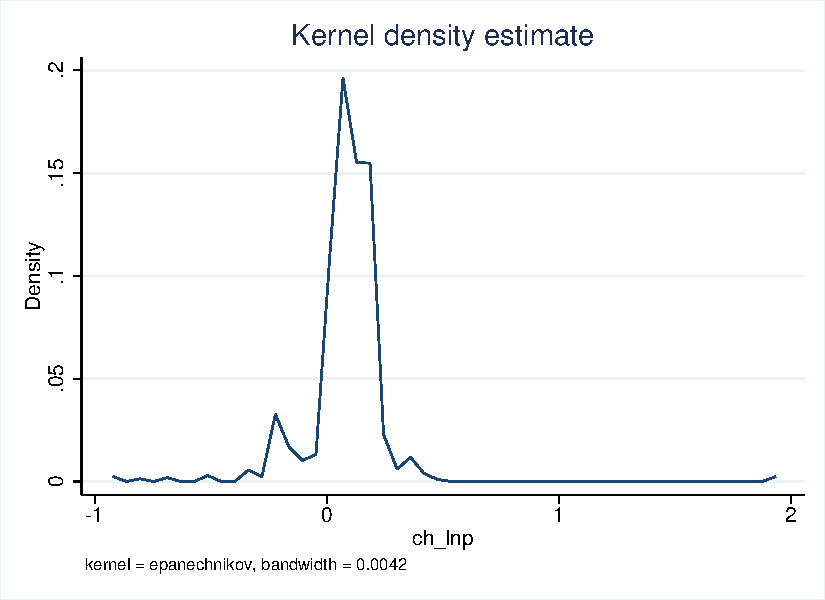
\includegraphics[width=3in]{ch_lnp_dens.pdf}
}
\end{frame}

\begin{frame}{Eat24 Means: Percent Change}
\Wider{
\centering
\tiny
{
\def\sym#1{\ifmmode^{#1}\else\(^{#1}\)\fi}
\begin{tabular}{l*{7}{c}}
\hline\hline
                    &\multicolumn{1}{c}{NYC Large}&\multicolumn{1}{c}{NYC Small}&\multicolumn{1}{c}{NYC MSA}&\multicolumn{1}{c}{MA}&\multicolumn{1}{c}{Upstate}&\multicolumn{1}{c}{NJ}&\multicolumn{1}{c}{PA}\\
\hline
Jul-Apr             &       0.453         &       0.291         &       0.556         &      0.0246         &      -0.278         &       0.106         &       0.141         \\
                    &     (3.958)         &     (2.975)         &     (3.396)         &     (2.747)         &     (2.865)         &     (5.122)         &     (5.292)         \\
[1em]
Oct-Jul             &       0.124         &       0.207         &      0.0123         &       0.206         &      -0.232         &       0.239         &       0.158         \\
                    &     (2.909)         &     (3.625)         &     (0.623)         &     (3.331)         &     (3.628)         &     (2.670)         &     (1.906)         \\
[1em]
Jan-Oct             &       0.579         &       0.266         &      0.0964         &       0.545         &       0.118         &       0.217         &       0.402         \\
                    &     (4.364)         &     (2.953)         &     (6.325)         &     (2.954)         &     (1.217)         &     (4.184)         &     (3.360)         \\
[1em]
Feb-Jan             &       0.147         &       0.103         &      0.0654         &      0.0882         &           0         &     -0.0222         &      0.0704         \\
                    &     (1.528)         &     (1.654)         &     (1.383)         &     (1.510)         &         (0)         &     (1.447)         &     (1.647)         \\
[1em]
Mar-Feb             &      0.0350         &      0.0899         &       0.174         &      0.0889         &           0         &      0.0628         &      0.0161         \\
                    &     (0.771)         &     (2.867)         &     (1.580)         &     (1.680)         &         (0)         &     (1.717)         &     (0.917)         \\
\hline
Obs        &       33791         &      238418         &       40072         &      128614         &       20234         &      147993         &      114114         \\
\hline\hline
%\multicolumn{8}{l}{\footnotesize mean coefficients; sd in parentheses}\\
%\multicolumn{8}{l}{\footnotesize \sym{*} \(p<0.05\), \sym{**} \(p<0.01\), \sym{***} \(p<0.001\)}\\
\end{tabular}
}

}
\end{frame}


\begin{frame}{Geocoded Yelp Means: Percent Change}
\Wider{
\centering
\tiny
{
\def\sym#1{\ifmmode^{#1}\else\(^{#1}\)\fi}
\begin{tabular}{l*{8}{c}}
\hline\hline
                    &\multicolumn{1}{c}{NYC}&\multicolumn{1}{c}{NYC MSA}&\multicolumn{1}{c}{MA}&\multicolumn{1}{c}{NY Upstate}&\multicolumn{1}{c}{CT}&\multicolumn{1}{c}{VT}&\multicolumn{1}{c}{NJ}&\multicolumn{1}{c}{PA}\\
\hline
Jul-Apr             &       0.139         &      0.0945         &      0.0777         &      0.0784         &      0.0753         &     -0.0356         &       0.111         &       0.111         \\
                    &     (2.396)         &     (3.923)         &     (2.336)         &     (2.319)         &     (3.355)         &     (1.270)         &     (4.907)         &     (4.184)         \\
[1em]
Oct-Jul             &       0.118         &      0.0376         &       0.116         &      0.0528         &       0.151         &       0.522         &      0.0768         &      0.0839         \\
                    &     (3.052)         &     (3.033)         &     (2.401)         &     (2.629)         &     (3.938)         &     (3.540)         &     (2.435)         &     (3.146)         \\
[1em]
Jan-Oct             &       0.202         &      0.0102         &       0.256         &      0.0353         &     0.00663         &      0.0210         &       0.170         &       0.173         \\
                    &     (3.774)         &     (2.944)         &     (2.877)         &     (1.187)         &     (0.241)         &     (1.319)         &     (4.594)         &     (2.980)         \\
[1em]
Feb-Jan             &      0.0662         &      0.0529         &      0.0351         &      0.0230         &           0         &           0         &      0.0327         &      0.0360         \\
                    &     (1.789)         &     (1.224)         &     (1.239)         &     (1.589)         &         (0)         &         (0)         &     (1.898)         &     (1.121)         \\
[1em]
Mar-Feb             &      0.0730         &      0.0943         &      0.0369         &      0.0371         &      0.0247         &      0.0239         &      0.0148         &      0.0168         \\
                    &     (2.879)         &     (1.179)         &     (2.376)         &     (0.770)         &     (0.661)         &     (0.602)         &     (1.918)         &     (1.765)         \\
\hline
Obs        &     1074449         &      219822         &      517650         &      154847         &       17160         &       18017         &      625056         &      443474         \\
\hline\hline
%\multicolumn{9}{l}{\footnotesize mean coefficients; sd in parentheses}\\
%\multicolumn{9}{l}{\footnotesize \sym{*} \(p<0.05\), \sym{**} \(p<0.01\), \sym{***} \(p<0.001\)}\\
\end{tabular}
}

}
\end{frame}


\begin{frame}{Grubhub Means: Percent Change}
\centering
\tiny
{
\def\sym#1{\ifmmode^{#1}\else\(^{#1}\)\fi}
\begin{tabular}{l*{8}{c}}
\hline\hline
                    &\multicolumn{1}{c}{NYC Large}&\multicolumn{1}{c}{NYC Small}&\multicolumn{1}{c}{NYC MSA}&\multicolumn{1}{c}{MA}&\multicolumn{1}{c}{Upstate}&\multicolumn{1}{c}{CT}&\multicolumn{1}{c}{NJ}&\multicolumn{1}{c}{PA}\\
\hline
Jan-Dec             &       0.321         &       0.267         &       0.237         &       0.281         &      0.0701         &      0.0322         &       0.112         &       0.446         \\
                    &     (2.078)         &     (2.840)         &     (2.213)         &     (2.096)         &     (2.297)         &     (2.733)         &     (1.870)         &     (4.438)         \\
[1em]
Feb-Jan             &       0.293         &       0.388         &       0.181         &       0.370         &       0.454         &      0.0253         &       0.217         &       0.264         \\
                    &     (2.612)         &     (3.094)         &     (2.091)         &     (2.618)         &     (3.366)         &     (1.668)         &     (2.557)         &     (2.786)         \\
[1em]
Mar-Feb             &       0.534         &       0.234         &       0.104         &       0.108         &       0.182         &      0.0965         &      0.0858         &       0.120         \\
                    &     (3.673)         &     (2.572)         &     (1.731)         &     (2.117)         &     (3.077)         &     (4.297)         &     (2.154)         &     (1.886)         \\
\hline
Obs        &       82115         &      521764         &      119421         &      143102         &       55084         &       22986         &      217892         &      192193         \\
\hline\hline
%\multicolumn{9}{l}{\footnotesize mean coefficients; sd in parentheses}\\
%\multicolumn{9}{l}{\footnotesize \sym{*} \(p<0.05\), \sym{**} \(p<0.01\), \sym{***} \(p<0.001\)}\\
\end{tabular}
}


\end{frame}

\begin{frame}{Grubhub Geocoded Means: Percent Change}
\centering
\tiny
{
\def\sym#1{\ifmmode^{#1}\else\(^{#1}\)\fi}
\begin{tabular}{l*{8}{c}}
\hline\hline
                    &\multicolumn{1}{c}{NYC Large}&\multicolumn{1}{c}{NYC Small}&\multicolumn{1}{c}{NYC MSA}&\multicolumn{1}{c}{MA}&\multicolumn{1}{c}{Upstate}&\multicolumn{1}{c}{CT}&\multicolumn{1}{c}{NJ}&\multicolumn{1}{c}{PA}\\
\hline
Dec-Jan             &       0.578         &       0.293         &       0.349         &       0.287         &     0.00694         &       0.178         &      0.0373         &       0.418         \\
                    &                     &                     &                     &                     &                     &                     &                     &                     \\
[1em]
Jan-Feb             &       0.337         &       0.430         &       0.177         &       0.208         &       0.426         &       0.179         &       0.183         &       0.256         \\
                    &                     &                     &                     &                     &                     &                     &                     &                     \\
[1em]
Feb-Mar             &       0.378         &       0.257         &       0.108         &       0.141         &       0.177         &       0.174         &      0.0706         &       0.182         \\
                    &                     &                     &                     &                     &                     &                     &                     &                     \\
[1em]
Mar-Apr             &       0.192         &       0.170         &       0.239         &       0.180         &       0.315         &       0.181         &       0.211         &       0.253         \\
                    &                     &                     &                     &                     &                     &                     &                     &                     \\
[1em]
Dec-Apr             &       1.485         &       1.152         &       0.867         &       0.832         &       0.911         &       0.705         &       0.498         &       1.109         \\
                    &                     &                     &                     &                     &                     &                     &                     &                     \\
\hline
Observations        &      101454         &      591318         &      134535         &      321582         &       71654         &       87386         &      522212         &      425472         \\
\hline\hline
\multicolumn{9}{l}{\footnotesize mean coefficients; se in parentheses}\\
\multicolumn{9}{l}{\footnotesize \sym{*} \(p<0.05\), \sym{**} \(p<0.01\), \sym{***} \(p<0.001\)}\\
\end{tabular}
}


\end{frame}

\begin{frame}{Grubhub Geocoded Means Rest Level: Percent Change}
\centering
\tiny
{
\def\sym#1{\ifmmode^{#1}\else\(^{#1}\)\fi}
\begin{tabular}{l*{8}{c}}
\hline\hline
                    &\multicolumn{1}{c}{NYC Large}&\multicolumn{1}{c}{NYC Small}&\multicolumn{1}{c}{NYC MSA}&\multicolumn{1}{c}{MA}&\multicolumn{1}{c}{Upstate}&\multicolumn{1}{c}{CT}&\multicolumn{1}{c}{NJ}&\multicolumn{1}{c}{PA}\\
\hline
Dec-Jan             &       0.427         &       0.373         &       0.430         &       0.209         &       0.215         &       0.255         &       0.161         &       0.511         \\
                    &                     &                     &                     &                     &                     &                     &                     &                     \\
[1em]
Jan-Feb             &       0.379         &       0.501         &       0.235         &       0.181         &       0.420         &       0.425         &       0.277         &       0.386         \\
                    &                     &                     &                     &                     &                     &                     &                     &                     \\
[1em]
Feb-Mar             &       0.314         &       0.275         &       0.151         &       0.321         &       0.170         &       0.125         &      0.0647         &       0.193         \\
                    &                     &                     &                     &                     &                     &                     &                     &                     \\
[1em]
Mar-Apr             &       0.350         &       0.235         &       0.276         &       0.205         &       0.392         &      0.0837         &       0.200         &       0.271         \\
                    &                     &                     &                     &                     &                     &                     &                     &                     \\
[1em]
Dec-Apr             &       1.470         &       1.385         &       1.093         &       0.915         &       1.198         &       0.888         &       0.702         &       1.360         \\
                    &                     &                     &                     &                     &                     &                     &                     &                     \\
\hline
Observations        &        1020         &        5216         &         928         &        2748         &         636         &         804         &        4064         &        3136         \\
\hline\hline
\multicolumn{9}{l}{\footnotesize mean coefficients; se in parentheses}\\
\multicolumn{9}{l}{\footnotesize \sym{*} \(p<0.05\), \sym{**} \(p<0.01\), \sym{***} \(p<0.001\)}\\
\end{tabular}
}


\end{frame}

\begin{frame}{Quality Means: Yelp}
\centering
\tiny
{
\def\sym#1{\ifmmode^{#1}\else\(^{#1}\)\fi}
\begin{tabular}{l*{6}{c}}
\hline\hline
                    &\multicolumn{1}{c}{NYC}&\multicolumn{1}{c}{NYC MSA}&\multicolumn{1}{c}{MA}&\multicolumn{1}{c}{Upstate}&\multicolumn{1}{c}{NJ}&\multicolumn{1}{c}{PA}\\
\hline
Apr-Jul             &      -0.476         &      -0.542         &       0.227         &      -0.386         &      -1.078         &      -0.142         \\
                    &     (15.46)         &     (13.00)         &     (13.59)         &     (11.84)         &     (13.54)         &     (12.43)         \\
[1em]
Jul-Oct             &      -0.894         &      -1.460         &      -0.615         &       0.199         &      -1.052         &      -0.821         \\
                    &     (15.38)         &     (14.36)         &     (14.18)         &     (12.73)         &     (13.02)         &     (12.92)         \\
[1em]
Oct-Jan             &       0.294         &       0.643         &       0.516         &       0.546         &       0.161         &      -0.107         \\
                    &     (14.61)         &     (13.44)         &     (13.55)         &     (10.58)         &     (13.04)         &     (12.70)         \\
[1em]
Jan-Apr             &      -0.274         &       0.130         &      -0.161         &      -0.106         &       0.471         &      -0.439         \\
                    &     (14.53)         &     (12.85)         &     (13.65)         &     (11.11)         &     (13.10)         &     (12.61)         \\
\hline
Observations        &       13656         &        1817         &        5706         &        1460         &        5344         &        3992         \\
\hline\hline
\multicolumn{7}{l}{\footnotesize mean coefficients; sd in parentheses}\\
\multicolumn{7}{l}{\footnotesize \sym{*} \(p<0.05\), \sym{**} \(p<0.01\), \sym{***} \(p<0.001\)}\\
\end{tabular}
}


\end{frame}

\begin{frame}{Yelp: Price Pass Through of a 10$\%$ MW Increase}
\Wider{

\centering
\tiny
{
\def\sym#1{\ifmmode^{#1}\else\(^{#1}\)\fi}
\begin{tabular}{l*{7}{c}}
\hline\hline
                    &\multicolumn{1}{c}{(1)}&\multicolumn{1}{c}{(2)}&\multicolumn{1}{c}{(3)}&\multicolumn{1}{c}{(4)}&\multicolumn{1}{c}{(5)}&\multicolumn{1}{c}{(6)}&\multicolumn{1}{c}{(7)}\\
                    &\multicolumn{1}{c}{RUSA}&\multicolumn{1}{c}{RUSA}&\multicolumn{1}{c}{RUSA}&\multicolumn{1}{c}{RUSA+Eat24}&\multicolumn{1}{c}{Geo}&\multicolumn{1}{c}{Geo}&\multicolumn{1}{c}{Geo+Eat24}\\
\hline
$\Delta Ln(mw_{Jan-Oct}) $&      0.0914\sym{**} &      0.0878         &      0.0946\sym{*}  &       0.0055         &       0.130\sym{***}&      0.0641\sym{***}&     0.00557         \\
                    &    (0.0248)         &    (0.0474)         &    (0.0477)         &    (0.1073)         &    (0.0137)         &    (0.0109)         &    (0.0266)         \\
[1em]
$\Delta Ln(mw_{Feb-Jan}) $&                     &      0.0543\sym{**} &      0.0611\sym{**} &    0.0489         &                     &      0.0594\sym{***}&      0.0766\sym{**} \\
                    &                     &    (0.0200)         &    (0.0209)         &    (0.0511)         &                     &   (0.00968)         &    (0.0155)         \\
[1em]
$\Delta Ln(mw_{Mar-Feb}) $&                     &      0.0638\sym{**} &      0.0706\sym{**} &           0.0315         &                     &      0.0756\sym{***}&      0.0888\sym{**} \\
                    &                     &    (0.0231)         &    (0.0243)         &         (0.0316)         &                     &    (0.0119)         &    (0.0362)         \\
\hline
Total & 0.091 & 0.206 & 0.226 & 0.086 & 0.130 & 0.202 & 0.171 \\
Controls & Yes & No & Yes & Yes & No & No & No \\
Obs        &     1408780         &     1878374         &     1878374         &      782051         &     1968874         &     3281458         &     1099284         \\
\hline\hline
\multicolumn{8}{l}{\footnotesize Standard errors in parentheses}\\
\multicolumn{8}{l}{\footnotesize \sym{*} \(p<.10\), \sym{**} \(p<.05\), \sym{***} \(p<.001\)}\\
\end{tabular}
}

}

\footnotesize
\begin{dmath}
\Delta \ln p_{ijkt} = \sum_{h=0}^{2}w_h \Delta \ln mw_{kt-h}  + \boldsymbol{X}_j \boldsymbol{\lambda} + \epsilon_k + \epsilon_t + \epsilon_{ijkt}
\end{dmath}

\end{frame}

\begin{frame}{Yelp Rests: Price Pass Through of a 10$\%$ MW Increase}
\Wider{
\centering
\tiny
{
\def\sym#1{\ifmmode^{#1}\else\(^{#1}\)\fi}
\begin{tabular}{l*{5}{c}}
\hline\hline
                    &\multicolumn{1}{c}{(1)}&\multicolumn{1}{c}{(2)}&\multicolumn{1}{c}{(3)}&\multicolumn{1}{c}{(4)}&\multicolumn{1}{c}{(5)}\\
                    &\multicolumn{1}{c}{(mean) ch\_lnp}&\multicolumn{1}{c}{(mean) ch\_lnp}&\multicolumn{1}{c}{(mean) ch\_lnp}&\multicolumn{1}{c}{(mean) ch\_lnp}&\multicolumn{1}{c}{(mean) ch\_lnp}\\
\hline
 $ Apr-Jul $        &      0.0461         &      0.0832\sym{**} &       0.310\sym{**} &      0.0120         &       0.111         \\
                    &    (0.0294)         &    (0.0215)         &     (0.114)         &     (0.143)         &     (0.339)         \\
[1em]
 $ Jul-Oct $        &       0.115         &      0.0764         &       0.639\sym{**} &     -0.0108         &      -0.296         \\
                    &    (0.0698)         &    (0.0726)         &     (0.192)         &     (0.280)         &     (0.678)         \\
[1em]
 $ Oct-Jan $        &       0.191\sym{**} &       0.202\sym{**} &       0.451\sym{**} &     -0.0695         &       0.105         \\
                    &    (0.0483)         &    (0.0573)         &     (0.127)         &     (0.136)         &     (0.361)         \\
[1em]
 $ Jan-Apr $        &       0.157\sym{**} &       0.142\sym{*}  &       0.435\sym{**} &       0.368         &       0.408         \\
                    &    (0.0602)         &    (0.0556)         &     (0.131)         &     (0.192)         &     (0.483)         \\
\hline
Observations        &       35460         &       21204         &        9080         &        4368         &        2468         \\
\hline\hline
\multicolumn{6}{l}{\footnotesize Standard errors in parentheses}\\
\multicolumn{6}{l}{\footnotesize \sym{*} \(p<.10\), \sym{**} \(p<.05\), \sym{***} \(p<.001\)}\\
\end{tabular}
}

}
\end{frame}

\begin{frame}{Grubhub: Price Pass Through of a 10$\%$ MW Increase}
\Wider{
\centering
\tiny
{
\def\sym#1{\ifmmode^{#1}\else\(^{#1}\)\fi}
\begin{tabular}{l*{3}{c}}
\hline\hline
                    &\multicolumn{1}{c}{(1)}&\multicolumn{1}{c}{(2)}&\multicolumn{1}{c}{(3)}\\
%                    &\multicolumn{1}{c}{ch\_lnp}&\multicolumn{1}{c}{ch\_lnp}&\multicolumn{1}{c}{ch\_lnp}\\
\hline
$\Delta Ln(mw_{Jan-Dec}) $&       0.168\sym{***}&       0.140\sym{***}&       0.207\sym{***}\\
                    &    (0.0110)         &    (0.0135)         &    (0.0169)         \\
[1em]
$\Delta Ln(mw_{Feb-Jan}) $&       0.225\sym{***}&       0.219\sym{**} &       0.285\sym{**} \\
                    &    (0.0230)         &    (0.0595)         &    (0.0671)         \\
[1em]
$\Delta Ln(mw_{Mar-Feb}) $&       0.153\sym{***}&       0.255\sym{**} &       0.321\sym{**} \\
                    &    (0.0196)         &    (0.0632)         &    (0.0783)         \\
\hline
Total & 0.395 & 0.614 & 0.813 \\
Controls & No & No & Yes \\
FE & No & Yes & Yes \\
Observations        &     1465718         &     1465718         &     1465718         \\
\hline\hline
\multicolumn{4}{l}{\footnotesize Standard errors in parentheses}\\
\multicolumn{4}{l}{\footnotesize \sym{*} \(p<.10\), \sym{**} \(p<.05\), \sym{***} \(p<.001\)}\\
\end{tabular}
}

}
\end{frame}

\begin{frame}{Grubhub Rest: Price Pass Through of a 10$\%$ MW Increase}
\Wider{
\centering
\tiny
{
\def\sym#1{\ifmmode^{#1}\else\(^{#1}\)\fi}
\begin{tabular}{l*{3}{c}}
\hline\hline
                    &\multicolumn{1}{c}{(1)}&\multicolumn{1}{c}{(2)}&\multicolumn{1}{c}{(3)}\\
                    &\multicolumn{1}{c}{(mean) ch\_lnp}&\multicolumn{1}{c}{(mean) ch\_lnp}&\multicolumn{1}{c}{(mean) ch\_lnp}\\
\hline
 $ Dec-Jan $        &       0.212\sym{***}&       0.193\sym{***}&       0.201\sym{***}\\
                    &    (0.0145)         &   (0.00974)         &   (0.00549)         \\
[1em]
 $ Jan-Feb $        &       0.252\sym{***}&       0.226\sym{**} &       0.263\sym{***}\\
                    &    (0.0116)         &    (0.0481)         &    (0.0306)         \\
[1em]
 $ Feb-Mar $        &       0.160\sym{***}&       0.240\sym{**} &       0.288\sym{***}\\
                    &    (0.0208)         &    (0.0421)         &    (0.0462)         \\
[1em]
 $ Mar-April $      &       0.149\sym{***}&       0.171\sym{**} &       0.179\sym{**} \\
                    &    (0.0190)         &    (0.0508)         &    (0.0633)         \\
\hline
Observations        &       18552         &       18552         &       12940         \\
\hline\hline
\multicolumn{4}{l}{\footnotesize Standard errors in parentheses}\\
\multicolumn{4}{l}{\footnotesize \sym{*} \(p<.10\), \sym{**} \(p<.05\), \sym{***} \(p<.001\)}\\
\end{tabular}
}

}
\end{frame}

\begin{frame}{Grubhub Rest: Price Pass Through of a 10$\%$ MW Increase}
\Wider{
\centering
\tiny
{
\def\sym#1{\ifmmode^{#1}\else\(^{#1}\)\fi}
\begin{tabular}{l*{7}{c}}
\hline\hline
                    &\multicolumn{1}{c}{(1)}&\multicolumn{1}{c}{(2)}&\multicolumn{1}{c}{(3)}&\multicolumn{1}{c}{(4)}&\multicolumn{1}{c}{(5)}&\multicolumn{1}{c}{(6)}&\multicolumn{1}{c}{(7)}\\
                    &\multicolumn{1}{c}{Popular}&\multicolumn{1}{c}{Side}&\multicolumn{1}{c}{Sandwich}&\multicolumn{1}{c}{Pizza}&\multicolumn{1}{c}{Entre}&\multicolumn{1}{c}{Desert}&\multicolumn{1}{c}{Drink}\\
\hline
$ Dec-Jan $         &       0.179\sym{***}&       0.165\sym{***}&       0.210\sym{***}&       0.141\sym{*}  &       0.147\sym{***}&       0.126\sym{**} &       0.166\sym{***}\\
                    &   (0.00429)         &    (0.0132)         &   (0.00441)         &    (0.0523)         &   (0.00221)         &    (0.0162)         &   (0.00343)         \\
[1em]
 $ Jan-Feb $        &       0.231\sym{***}&       0.200\sym{**} &       0.220\sym{***}&       0.182\sym{**} &       0.155\sym{***}&       0.114\sym{**} &       0.211\sym{**} \\
                    &   (0.00339)         &    (0.0530)         &   (0.00548)         &    (0.0366)         &    (0.0132)         &    (0.0224)         &    (0.0290)         \\
[1em]
 $ Feb-Mar $        &       0.143\sym{***}&       0.260\sym{***}&       0.231\sym{***}&       0.162         &      0.0504\sym{**} &       0.102\sym{**} &      0.0354         \\
                    &    (0.0145)         &    (0.0189)         &    (0.0141)         &     (0.141)         &   (0.00604)         &    (0.0228)         &    (0.0409)         \\
[1em]
 $ Mar-April $      &      0.0631\sym{**} &      0.0670\sym{**} &      0.0245         &      -0.149\sym{**} &      0.0129         &      0.0142         &    -0.00191         \\
                    &    (0.0150)         &    (0.0168)         &    (0.0369)         &    (0.0364)         &   (0.00714)         &    (0.0241)         &    (0.0178)         \\
\hline
Observations        &       95389         &      212921         &      227011         &       83246         &      324712         &       39854         &      127038         \\
\hline\hline
\multicolumn{8}{l}{\footnotesize Standard errors in parentheses}\\
\multicolumn{8}{l}{\footnotesize \sym{*} \(p<.10\), \sym{**} \(p<.05\), \sym{***} \(p<.001\)}\\
\end{tabular}
}

}
\end{frame}

\begin{frame}{Yelp Rest: Price Pass Through of a 10$\%$ MW Increase}
\Wider{
\centering
\tiny
{
\def\sym#1{\ifmmode^{#1}\else\(^{#1}\)\fi}
\begin{tabular}{l*{6}{c}}
\hline\hline
                    &\multicolumn{1}{c}{(1)}&\multicolumn{1}{c}{(2)}&\multicolumn{1}{c}{(3)}&\multicolumn{1}{c}{(4)}&\multicolumn{1}{c}{(5)}&\multicolumn{1}{c}{(6)}\\
                    &\multicolumn{1}{c}{Low Sales}&\multicolumn{1}{c}{High Sales}&\multicolumn{1}{c}{Low Emps}&\multicolumn{1}{c}{High Emps}&\multicolumn{1}{c}{Low Stars}&\multicolumn{1}{c}{High Stars}\\
\hline
$ Jul-Oct $         &     -0.0849         &      -0.164         &       0.462         &     -0.0870         &      -0.182         &     -0.0284         \\
                    &    (0.0790)         &     (0.137)         &     (0.315)         &     (0.152)         &     (0.104)         &    (0.0978)         \\
[1em]
$ Oct-Jan $         &      0.0701         &     -0.0180         &       0.480\sym{*}  &     -0.0153         &       0.141         &      0.0135         \\
                    &    (0.0663)         &    (0.0888)         &     (0.220)         &     (0.100)         &    (0.0924)         &    (0.0648)         \\
[1em]
$ Jan-Apr $         &       0.121\sym{**} &       0.330\sym{**} &       0.503         &       0.323\sym{**} &       0.208         &     -0.0335         \\
                    &    (0.0397)         &     (0.101)         &     (0.246)         &     (0.109)         &     (0.115)         &     (0.110)         \\
\hline
Observations        &        5332         &        5960         &        5940         &        7368         &        5376         &       10676         \\
\hline\hline
\multicolumn{7}{l}{\footnotesize Standard errors in parentheses}\\
\multicolumn{7}{l}{\footnotesize \sym{*} \(p<.10\), \sym{**} \(p<.05\), \sym{***} \(p<.001\)}\\
\end{tabular}
}

}
\end{frame}

\begin{frame}{Grubhub Item: Price Pass Through of a 10$\%$ MW Increase}
\Wider{
\centering
\tiny
{
\def\sym#1{\ifmmode^{#1}\else\(^{#1}\)\fi}
\begin{tabular}{l*{6}{c}}
\hline\hline
                    &\multicolumn{1}{c}{(1)}&\multicolumn{1}{c}{(2)}&\multicolumn{1}{c}{(3)}&\multicolumn{1}{c}{(4)}&\multicolumn{1}{c}{(5)}&\multicolumn{1}{c}{(6)}\\
                    &\multicolumn{1}{c}{Low Sales}&\multicolumn{1}{c}{High Sales}&\multicolumn{1}{c}{Low Emps}&\multicolumn{1}{c}{High Emps}&\multicolumn{1}{c}{Low Price}&\multicolumn{1}{c}{High Price}\\
\hline
$ Dec-Jan $         &      0.0736\sym{**} &       0.272\sym{***}&       0.116\sym{***}&       0.199\sym{***}&       0.288\sym{***}&       0.182\sym{***}\\
                    &    (0.0301)         &   (0.00410)         &    (0.0103)         &    (0.0182)         &   (0.00866)         &   (0.00684)         \\
[1em]
 $ Jan-Feb $        &       0.192\sym{**} &       0.301\sym{*}  &       0.163\sym{**} &       0.229         &       0.297\sym{***}&       0.235\sym{***}\\
                    &    (0.0375)         &     (0.139)         &    (0.0301)         &     (0.168)         &    (0.0151)         &    (0.0342)         \\
[1em]
 $ Feb-Mar $        &       0.175\sym{***}&       0.293\sym{**} &       0.138\sym{***}&       0.290\sym{*}  &       0.375\sym{**} &       0.235\sym{**} \\
                    &    (0.0276)         &     (0.113)         &    (0.0196)         &     (0.120)         &    (0.0709)         &    (0.0592)         \\
[1em]
 $ Mar-April $      &       0.125         &       0.254\sym{*}  &      0.0845         &       0.282\sym{*}  &       0.114\sym{*}  &      0.0905\sym{**} \\
                    &    (0.0978)         &     (0.129)         &    (0.0968)         &     (0.130)         &    (0.0566)         &    (0.0269)         \\
\hline
Observations        &        3376         &        3420         &        4232         &        1700         &        3488         &        3824         \\
\hline\hline
\multicolumn{7}{l}{\footnotesize Standard errors in parentheses}\\
\multicolumn{7}{l}{\footnotesize \sym{*} \(p<.10\), \sym{**} \(p<.05\), \sym{***} \(p<.001\)}\\
\end{tabular}
}

}
\end{frame}

\begin{frame}{Yelp: Changes in Quality}
\Wider{
\centering
\tiny
\begin{center}
\begin{tabular}{lcccccccccccc}
\hline  & \multicolumn{2}{c}{All} & \multicolumn{2}{c}{ $ 2.5 $ } & \multicolumn{2}{c}{ $ 3.0 $ } & \multicolumn{2}{c}{ $ 3.5 $ } & \multicolumn{2}{c}{ $ 4.0 $ } & \multicolumn{2}{c}{ $ 4.5$ }\\
 & (1) & (2) & (3) & (4) & (5) & (6) & (7) & (8) & (9) & (10) & (11) & (12)\\
\hline  $ Jul16-Oct16 $  & -0.083 & -0.082 & -1.459 & -1.478 & -0.930 & -0.940 & 0.041 & 0.041 & 1.304 & 1.296 & -0.165 & -0.160\\
 & (0.198) & (0.196) & (1.208) & (1.218) & (0.743) & (0.743) & (0.242) & (0.234) & (0.793) & (0.790) & (0.820) & (0.825)\\
 $ Oct16-Jan17 $  & -0.110 & -0.102 & -0.883 & -0.904 & -1.966* & -1.983* & -0.335 & -0.326 & 1.479* & 1.489* & 1.097 & 1.087\\
 & (0.166) & (0.160) & (2.221) & (2.238) & (0.867) & (0.868) & (0.207) & (0.214) & (0.539) & (0.539) & (0.533) & (0.538)\\
 $ Jan17-Apr17 $  & -0.415 & -0.407 & -2.296 & -2.259 & -1.171 & -1.183 & -0.796* & -0.785* & 0.912 & 0.922 & 0.372 & 0.362\\
 & (0.354) & (0.359) & (1.751) & (1.745) & (1.201) & (1.204) & (0.327) & (0.348) & (0.686) & (0.679) & (0.563) & (0.569)\\
 \textit{Change Price}  &  & -0.028 &  & -0.105* &  & 0.037 &  & -0.032 &  & -0.003 &  & -0.033\\
 &  & (0.025) &  & (0.049) &  & (0.024) &  & (0.031) &  & (0.056) &  & (0.032)\\
\hline \textit{Total \% Change Stars} & -0.526 & -0.509 & -3.179 & -3.163 & -3.136* & -3.166* & -1.131*** & -1.111** & 2.391** & 2.411** & 1.468* & 1.45*\\
  & (0.451) & (0.453) & (3.969) & (3.981) & (2.021) & (2.028) & (0.486) & (0.518) & (1.185) & (1.178) & (1.008) & (1.02)\\
\hline  $ N $  & 6817 & 6815 & 625 & 625 & 1080 & 1080 & 1801 & 1800 & 1904 & 1903 & 982 & 982\\
 $ NxT $  & 27268 & 27260 & 2500 & 2500 & 4320 & 4320 & 7204 & 7200 & 7616 & 7612 & 3928 & 3928\\
\hline\end{tabular}\\
\begin{tiny}\ * $p<0$.1; ** $p<0$.05; *** $p<0$.01\end{tiny}\\
\end{center}

}
\end{frame}



\begin{frame}{Yelp: Border Effects}
\Wider{
\centering
\tiny
{
\def\sym#1{\ifmmode^{#1}\else\(^{#1}\)\fi}
\begin{tabular}{l*{4}{c}}
\hline\hline
                    &\multicolumn{1}{c}{(NJ)}&\multicolumn{1}{c}{(NJ)}&\multicolumn{1}{c}{(NJ)}&\multicolumn{1}{c}{(NY MSA)}\\
                    &\multicolumn{1}{c}{$Oct-Feb$}&\multicolumn{1}{c}{$Oct-Feb$}&\multicolumn{1}{c}{$Jul-Oct$}&\multicolumn{1}{c}{$Oct-Feb$}\\
\hline
Constant ($ \alpha_0 $)           &     .00261         &     .00268         &   -.000689         &     .00198         \\
                    &   (.00145)         &   (.00146)         &  (.000873)         &   (.00318)        \\
        [1em]
NYC ($ \alpha_1 $)     &    -.00339\sym{**}  &    -.00410\sym{**}  &     .00218\sym{**}  &       -.00589              \\
                    &   (.00160)         &   (.00161)         &  (.000961)         &                     (.00329)   \\
[1em]
Distance   ($\alpha_2$)            &   .0000454         &   .0000683         &  -.0000366         &                      .000245         \\
                    & (.0000566)         & (.0000568)         & (.0000339)         &                     (0.000168)      \\
%[1em]
%ny=0 $\times$ dist\_nynj\_bord&           0         &           0         &           0         &                     \\
%                    &         (.)         &         (.)         &         (.)         &                     \\
[1em]
NYC $\times$ Distance ($\alpha_3$)    &    .000350\sym{***}&    .000322\sym{***}&   .0000461         &     .000293\sym{*}                 \\
                    & (.0000678)         & (.0000679)         & (.0000405)         &                     (.000177)   \\
%Chain               &                     &    -0.00553\sym{*}  &    -0.00222         &                     \\
%                    &                     &   (0.00243)         &   (0.00145)         &                     \\
%[1em]
%LS                  &                     &    -0.00383\sym{***}&    -0.00113\sym{*}  &                     \\
%                    &                     &  (0.000907)         &  (0.000542)         &                     \\
%[1em]
%Employees           &                     &  -0.0000586         &   0.0000367         &                     \\
%                    &                     & (0.0000472)         & (0.0000282)         &                     \\
%[1em]
%Sales               &                     &    2.48e-09\sym{***}&    1.82e-11         &                     \\
%                    &                     &  (4.42e-10)         &  (2.64e-10)         &                     \\
%[1em]
%nyc                 &                     &                     &                     &    -0.00589         \\
%                    &                     &                     &                     &   (0.00329)         \\
%[1em]
%dist\_nyny\_bord      &                     &                     &                     &    0.000245         \\
%                    &                     &                     &                     &  (0.000168)         \\
%[1em]
%nyc=0 $\times$ dist\_nyny\_bord&                     &                     &                     &           0         \\
%                    &                     &                     &                     &         (.)         \\
%[1em]
%nyc=1 $\times$ dist\_nyny\_bord&                     &                     &                     &    0.000293         \\
%                    &                     &                     &                     &  (0.000177)         \\
%[1em]
 \\
\hline
Observations        &       80402         &       80402         &       80402         &       23368         \\
\hline\hline
%	\multicolumn{5}{l}{\footnotesize Standard errors in parentheses}\\
%	\multicolumn{5}{l}{\footnotesize \sym{*} \(p<0.05\), \sym{**} \(p<0.01\), \sym{***} \(p<0.001\)}\\
\end{tabular}
}

}

\small
$$
\begin{aligned}
\Delta \ln (p_{ij,Feb-Oct})  = & \alpha_0 + \alpha_1  \mathbbm{1}(NY=1)  \\
& + \alpha_2 D_{j} + \alpha_3[D_j * \mathbbm{1}(NY=1)]  \\
& +\gamma X_{ij}  + \epsilon_{ij} 
\end{aligned}
$$
\end{frame}

\begin{frame}{Yelp: Border Effects}
\tiny
{
\def\sym#1{\ifmmode^{#1}\else\(^{#1}\)\fi}
\begin{tabular}{l*{5}{c}}
\hline\hline
                    &\multicolumn{1}{c}{(1)}         &\multicolumn{1}{c}{(2)}         &\multicolumn{1}{c}{(3)}         &\multicolumn{1}{c}{(4)}         &\multicolumn{1}{c}{(5)}         \\
                    &        Yelp         &     Jul-Oct         &        NYNY         &          GH         &        NYNY         \\
\hline
\textbf{1}(NY)      &      0.0166         &    -0.00427         &                     &     -0.0398\sym{**} &                     \\
                    &    (0.0188)         &    (0.0140)         &                     &    (0.0160)         &                     \\
[1em]
Distance            &    -0.00157         &   -0.000127         &                     &     0.00135\sym{*}  &                     \\
                    &   (0.00106)         &  (0.000791)         &                     &  (0.000796)         &                     \\
[1em]
ny=0 $\times$ dist\_nynj\_bord&           0         &           0         &                     &           0         &                     \\
                    &         (.)         &         (.)         &                     &         (.)         &                     \\
[1em]
ny=1 $\times$ dist\_nynj\_bord&     0.00265\sym{*}  &    0.000817         &                     &     0.00173         &                     \\
                    &   (0.00136)         &   (0.00101)         &                     &   (0.00130)         &                     \\
[1em]
nyc                 &                     &                     &    -0.00712         &                     &    -0.00839         \\
                    &                     &                     &    (0.0198)         &                     &    (0.0142)         \\
[1em]
dist\_nyny\_bord      &                     &                     &   -0.000131         &                     &    0.000344         \\
                    &                     &                     &  (0.000625)         &                     &  (0.000553)         \\
[1em]
nyc=0 $\times$ dist\_nyny\_bord&                     &                     &           0         &                     &           0         \\
                    &                     &                     &         (.)         &                     &         (.)         \\
[1em]
nyc=1 $\times$ dist\_nyny\_bord&                     &                     &    0.000671         &                     &    0.000259         \\
                    &                     &                     &   (0.00203)         &                     &   (0.00142)         \\
[1em]
Constant            &     -0.0171         &     0.00202         &     0.00644         &      0.0262\sym{**} &      0.0146\sym{**} \\
                    &    (0.0172)         &    (0.0128)         &   (0.00848)         &    (0.0130)         &   (0.00704)         \\
\hline
Observations        &         896         &         896         &         439         &         499         &         184         \\
\hline\hline
\multicolumn{6}{l}{\footnotesize Standard errors in parentheses}\\
\multicolumn{6}{l}{\footnotesize \sym{*} \(p<.10\), \sym{**} \(p<.05\), \sym{***} \(p<.001\)}\\
\end{tabular}
}

\end{frame}


\begin{frame}{Grubhub: Border Effects}
\tiny
{
\def\sym#1{\ifmmode^{#1}\else\(^{#1}\)\fi}
\begin{tabular}{l*{2}{c}}
\hline\hline
                    &\multicolumn{1}{c}{(1)}&\multicolumn{1}{c}{(2)}\\
                    &\multicolumn{1}{c}{total\_chlnp}&\multicolumn{1}{c}{total\_chlnp}\\
\hline
\textbf{1}(NY)      &     -0.0196         &     -0.0113         \\
                    &    (0.0138)         &    (0.0196)         \\
[1em]
Distance            &  -0.0000298         &   -0.000461         \\
                    &  (0.000578)         &  (0.000951)         \\
[1em]
ny=0 $\times$ dist\_nynj\_bord&           0         &           0         \\
                    &         (.)         &         (.)         \\
[1em]
ny=1 $\times$ dist\_nynj\_bord&     0.00310\sym{**} &     0.00278         \\
                    &   (0.00117)         &   (0.00146)         \\
[1em]
chain               &                     &     -0.0148         \\
                    &                     &    (0.0266)         \\
[1em]
ls                  &                     &     0.00680         \\
                    &                     &   (0.00789)         \\
[1em]
employees           &                     &    -0.00319\sym{***}\\
                    &                     &  (0.000430)         \\
[1em]
sales               &                     &    3.84e-08\sym{***}\\
                    &                     &  (5.22e-09)         \\
[1em]
Constant            &     0.00592         &     0.00413         \\
                    &    (0.0102)         &    (0.0170)         \\
\hline
Observations        &         599         &         378         \\
\hline\hline
\multicolumn{3}{l}{\footnotesize Standard errors in parentheses}\\
\multicolumn{3}{l}{\footnotesize \sym{*} \(p<0.05\), \sym{**} \(p<0.01\), \sym{***} \(p<0.001\)}\\
\end{tabular}
}

\end{frame}

\end{spacing}
\end{document}











































